Solving sophisticated image analysis problems usually requires to apply a combination of different
algorithms to given data to extract desired results. In ImageJ this can be
accomplished by applying a sequence of plugins sequentially or in parallel to given image data and 
record a macro of the processing steps for later reuse. \mitobo extends ImageJ's support for such 
workflows formed by multiple plugins or operators, respectively, by featuring a graphical 
editor for simplified workflow design. The editor named {\tt Grappa}, which is the acronym for 
{\em {\bf \em Grap}hical {\bf \em P}rogramming Editor for {\bf \em A}lida}, can be invoked from the plugins menu.  

In Fig.~\ref{fig:grappa} a screenshot of the Grappa main window is shown. 
The window is basically separated into
the node selection menu on the left and the workbench area on the right. In the selection menu 
all \alida and \mitobo operators (and in ImageJ $2.0$ also a subset of its plugins) are 
available as processing nodes for Grappa. The nodes in the selection menu are arranged in a 
hierarchical ordering according to their package structure. 

Workflows can be designed in the workbench area on the right. It allows to instantiate different 
workflows each being linked to an individual tab of the workbench panel. Operator nodes can be
added to a workflow either by double-clicking on the operator name in the selection menu or by 
selecting an operator and afterwards clicking once on the position in the workflow tab where the 
operator node should be positioned. Nodes can easily be dragged and repositioned as well as 
resized by mouse actions. Once different nodes have been added to a workflow, edges
can be added between ports of different nodes with the mouse to define the flow of data and control. 
All edges
are directed, always connecting an output port of one node with an input port of another. Note
that on drawing edges Grappa performs type-checking, i.e.~only ports being associated with 
compatible parameter data types can be linked to each other.
\begin{center}
\begin{figure}[t]
\begin{center}
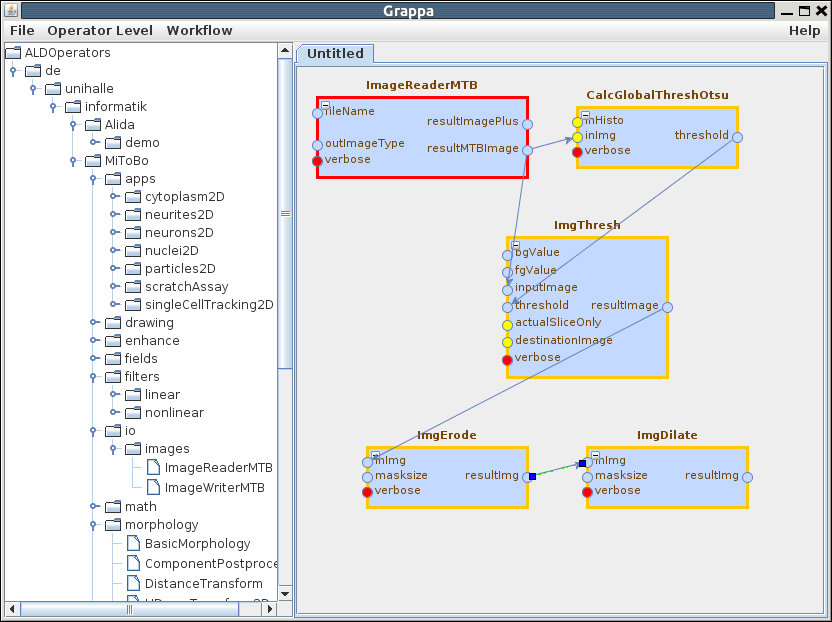
\includegraphics[width=0.85\textwidth]{../images/ScreenshotGrappa.png}
\caption{\label{fig:grappa}Screenshot of the graphical workflow editor Grappa.}
\end{center}
\end{figure}
\end{center}

\vspace*{-0.5cm}
For node configuration the mechanisms of the graphical operator runner (Sec.~\ref{sec:opRunImageJ})
are adopted. From the context menu of a node (which opens on right-clicking on the node) 
the option 'Configure\ldots' is available by which a graphical configuration window pops up.
The window is essentially identical to the control window which is displayed by the operator 
runner except that the control section is missing. All parameter values can easily be edited via
the graphical components of the window.

Nodes in a workflow can have different states indicated by the color of their border. Red framed
nodes are not ready for execution, i.e.~their configuration is not complete. If a node is readily
configured and can directly be executed its border has a yellow color, while nodes that are 
configured, however, require additional input data from preceeding operator nodes (like most of 
the nodes in Fig.~\ref{fig:grappa}) have an orange color. Prior to executing these orange nodes it
is, thus, necessary to execute the preceeding nodes first. Grappa takes care of such 
dependencies, i.e.~automatically executes nodes first from which result data is required for 
proper workflow or node execution.
After successful execution of a node its color 
changes to green indicating that result data is available. These data can graphically be examined 
via the node's context menu from which a result window can be opened. 
Note that Grappa updates the state of a node in 
real-time, i.e.~each change in its configuration or state is directly mirrored by its border color.

For executing a workflow Grappa offers different modes. Either a complete workflow can be 
executed or just a fraction of it up to a certain node. To run the complete workflow use the
corresponding item from Grappa's menubar or right-click on an empty place in the workflow tab and
select the related option from the context menu which is shown. To only partially run a workflow
select the corresponding option from the context menu of the node until which you would like to 
execute the workflow. Nodes having green color cannot be executed again until their configuration 
is changed.

Apart from the basic functionality for workflow design Grappa offers some additional convenience 
functions to simplify working with the editor. For example workflows can be saved to 
and read from disk. They can be renamed to meaningful names, and also a complete reset of a 
workflow in terms of deleting all nodes is possible. For more information on Grappa please refer
to the Alida documentation and its user and programmer guide.
